\chapter{Why All Writing Sounds the Same Now}

This lecture contains no literal board mathematics. There are no derivations on a blackboard, no symbolic manipulations, and no formulas to recover from a slide. But there is still a mathematical spine to the argument. Macfarlane keeps asking how one form of writing can answer one form of experience, and the host keeps sharpening that question until it becomes local and exact. The lecture therefore unfolds through distinctions, ladders, pipelines, scales, and transformations of agency. It begins with biography, pivots to light, moves into the minute mechanics of prose, widens into process and worldview, and closes with revision, precision, and the defense of distinctiveness against flattening.

\begin{remark}
The formulas in this chapter are schematic statements of structures the lecture makes explicitly in speech. They are not recovered lecture notation. We use them only where they clarify the formal logic of the talk.
\end{remark}

\section{Mountains, Light, and the Failure of Capture}

The lecture opens in the right place: not with doctrine, but with admiration and origin. The host asks where Macfarlane's sensitivity comes from, and Macfarlane answers in the language of training rather than talent. He grew up in mountains. Mountains sharpen sensation, demand alertness, and wear away the usual shell of the self. Danger is therefore not incidental background. It is one of the engines of perception.

The lecture's first causal chain may be written schematically as
\begin{equation}
\text{danger} \longrightarrow \text{alertness} \longrightarrow \text{openness} \longrightarrow \text{attention}.
\end{equation}
This is already more than autobiography. It is an account of how a writer gets formed. Brighter light, sharper snow, air felt like wire in the nose, risk assessment, bodily exposure: all of these become modes of noticing. Mountains do not merely supply scenery. They supply an education of the senses.

From that opening the host makes the first decisive pivot: ``Tell me about that obsession with light.'' He gives a fresh anecdote about a failed attempt to photograph a sunset from a plane, then the grief of realizing that the scene will fade in memory and may never become fully sayable. That grief matters. If we skip it, we lose the lecture's true motivating problem. Macfarlane does not begin from abstract aesthetics; he begins from the felt inadequacy of language before a particular intensity of seeing.

His answer comes in two stages. First, he intensifies the sunset in speech --- there was, as he says, almost a slaughter in it, something bloody and wild. Then he steps back and states the formal lesson. When the subject is light, language is always late.

The core opposition of the lecture appears here:
\begin{align}
\text{correspondence} &\not\Rightarrow \text{adequate writing of light},\\
\text{artifice} &\Rightarrow \text{evocation of perception}.
\end{align}
If we cling to correspondence, we remain trapped in a futile quest to make language meet the thing exactly. Macfarlane's recommendation is more radical and more liberating: abandon that quest. Once we stop insisting that words reproduce the scene point for point, we can let metaphor, distortion, and formal construction do their proper work.

\begin{definition}
By \emph{representation of perception} the lecture means not the thing in itself, but the thing as it arrives through a particular encounter: filtered by movement, mood, history, and attention.
\end{definition}

This is why the host's impressionist analogy lands so well. Monet is not trying to imprison the scene inside paint. He is painting the impression of the scene. Macfarlane makes the same move in prose. He even resists the verb ``capture,'' because to capture nature is already to imagine it as captive. A better verb is evoke. Once that distinction is in place, the lecture can move from light to a different medium in which form and movement are even more obviously inseparable: water.

\section{Water, Punctuation, and the Small Mechanics of Thought}

Water arrives not as a new topic but as the first sustained test of the anti-correspondence method. Macfarlane has spent years writing a river book, and from that long labor he draws a strong formal conclusion: there is no single grammar of water. That is the point on which the rest of the section turns.

The host is helpful here because he immediately grounds the abstraction. Rivers do not all move the same way. They can be still, pooled, meandering, straight, rapid. Once he says this, Macfarlane can sharpen the lesson:
\begin{equation}
\text{river language} \neq \text{fast language only}.
\end{equation}
That correction matters. ``Flow'' is too weak a metaphor if it collapses all waters into one prose texture. Flat lake water, turning river water, and wild rapid water require different rhythms, tones, and sentence structures.

In the lecture's own progression, the river taxonomy becomes a prose taxonomy:
\begin{itemize}
\item pooled or still water asks for delay, breadth, and pause,
\item meandering water permits drift, turn, and soft redirection,
\item straight water allows propulsion and line,
\item rapid water demands urgency, accumulation, and impact.
\end{itemize}

From there the talk narrows from large form to tiny operators. Macfarlane calls himself both a preposition obsessive and a punctuation obsessive. The dash comes first. A full stop, he says, bangs down a hard end. The dash remains liquid. Meaning can eddy backward through it or flow onward through it. This is not an ornament. It is a model of how syntax can manage motion without sealing it off.

The prepositions come next, and here the lecture becomes unusually exact. The preposition is not filler. It changes the whole metaphysical relation between writer and world:
\begin{equation}
\text{about river} \longrightarrow \text{with river} \longrightarrow \text{by river}.
\end{equation}
To write \emph{about} a river is to describe it as object. To write \emph{with} a river is already to grant it a kind of co-authorship, or at least co-presence in thought. To be written \emph{by} river goes further still. The writer becomes conduit, channel, medium. The host recognizes the force of this at once and restates it more plainly: almost as if the river becomes co-author. That restatement belongs in the notes, because the lecture repeatedly advances in just this way --- Macfarlane gives the pressure of the distinction, and the host compresses it into a more pedagogical sentence.

Rhythm is the next narrowing. Poetry teaches us to expect rhythm, but nonfiction, Macfarlane argues, also acts on what he calls the reader's ``mind's ear.'' It does not work only by proposition. It works by sound, pattern, cadence, and internal rhyme. That is why he spends so long on first lines. A first line has to do several jobs at once, and the lecture effectively gives us a simple model:
\begin{equation}
\text{first line} = \text{sound pattern} + \text{puzzle} + \text{conceptual opening}.
\end{equation}

``The wind was rising, so I went to the wood'' is the lecture's happiest instance. It gives us alliteration, rhythm, and a puzzle at once. Why go into the wood when the wind is rising? That is not merely pretty phrasing. It is a small narrative engine. By contrast, ``12{,}000 years ago, a river is born'' is, as the lecture says, less rhythmic but more ominous. It trades overt sound for temporal vastness and conceptual mystery.

Macfarlane then pushes even more finely into internal sound pattern. ``White as eyes'' and ``rises and flows'' begin to echo one another; the text starts to work on the reader before an argument has been laid out. This is the lecture's important reminder that nonfiction need not be flatly propositional simply because it is nonfiction.

At this point the groundwork has been laid. Water has become formal principle, punctuation and prepositions have been promoted to real operators, and rhythm has been restored to nonfiction. Now the host can ask the lecture's clearest local craft question.

\section{Writing Speed as a Formal Problem}

\subsection{Question \& Answer}

\paragraph{Question.} How do we write speed?

\paragraph{Answer.} Not by a crude rule such as ``make the sentences short.'' The lecture's answer is more precise. We write speed by building a syntax that tumbles, contracts, and denies the reader an easy place to rest.

Macfarlane does exactly what the host has earned the right to ask for: he produces an example. More than that, the lecture places the example itself on screen, which tells us something about the pedagogy. He is not merely describing fast prose in the abstract; he is pausing to inspect a specimen.

\begin{figure}[ht]
\centering

\includegraphics[width=0.92\textwidth]{lecture_17_figure_02.png}
\caption{On-screen river passage illustrating a syntax of speed and panic}
\end{figure}

The screenshot is important as evidence. It contains no visible equations or lecture diagrams; the prose block itself is the exhibit. The quotation is dense, accumulative, and almost unbroken. The eye meets pressure before the theory is even explained.

Macfarlane's explanation can be written compactly as
\begin{equation}
\#(\text{and}) \uparrow,\qquad \ell_{\text{clause}} \downarrow,\qquad a_{\text{verb}} \uparrow
\Longrightarrow \text{panic and speed} \uparrow.
\end{equation}
Here \(\ell_{\text{clause}}\) is average clause length, and \(a_{\text{verb}}\) denotes the pressure exerted by increasingly active verbs.

He also gives a crucial local equivalence:
\begin{equation}
\text{``and''} \sim \text{dash}.
\end{equation}
That is, in this kind of prose the conjunction does the work the dash was doing earlier. It keeps the line running. It prevents calm hierarchy. It refuses the stop-start composure of a sentence organized by full stops and neat subordination.

The derivation is simple, but it is exact. We can state it in the lecture's own order:
\begin{enumerate}
\item Start inside an already moving sentence rather than from a cleanly bounded clause.
\item Repeat ``and'' so that one unit keeps spilling into the next.
\item Let the clauses between conjunctions become shorter and quicker.
\item Increase the pressure of the verbs: slammed, exploded, punching, ramming, hauling.
\item Drop the article in ``river,'' so that the force ceases to feel like a named object and starts to feel like a medium acting everywhere at once.
\item Result: the reader becomes breathless, because the syntax withholds the ordinary points at which breath and hierarchy would be restored.
\end{enumerate}

The dropped article is a particularly strong small move. ``The river'' is a thing we can stand apart from. ``River'' feels more like agency, more like impact, less like scenery. A trivial grammatical subtraction changes the ontology of the scene.

Because the screen gives us only the prose block and not an analytic diagram, any diagram we add must remain visibly secondary. What follows is therefore an editorial reconstruction, not a recovered lecture graphic.

\begin{figure}[ht]
\centering
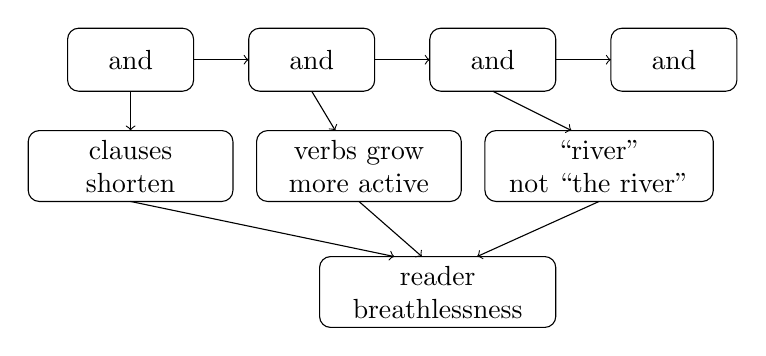
\begin{tikzpicture}[x=1cm,y=1cm]
\draw[rounded corners] (-5.2,1.2) rectangle (-3.6,2.0);
\node at (-4.4,1.6) {and};
\draw[rounded corners] (-2.9,1.2) rectangle (-1.3,2.0);
\node at (-2.1,1.6) {and};
\draw[rounded corners] (-0.6,1.2) rectangle (1.0,2.0);
\node at (0.2,1.6) {and};
\draw[rounded corners] (1.7,1.2) rectangle (3.3,2.0);
\node at (2.5,1.6) {and};

\draw[->] (-3.6,1.6) -- (-2.9,1.6);
\draw[->] (-1.3,1.6) -- (-0.6,1.6);
\draw[->] (1.0,1.6) -- (1.7,1.6);

\draw[rounded corners] (-5.7,-0.2) rectangle (-3.1,0.7);
\node[align=center] at (-4.4,0.25) {clauses\\shorten};

\draw[rounded corners] (-2.8,-0.2) rectangle (-0.2,0.7);
\node[align=center] at (-1.5,0.25) {verbs grow\\more active};

\draw[rounded corners] (0.1,-0.2) rectangle (3.0,0.7);
\node[align=center] at (1.55,0.25) {``river''\\not ``the river''};

\draw[rounded corners] (-2.0,-1.8) rectangle (1.0,-0.9);
\node[align=center] at (-0.5,-1.35) {reader\\breathlessness};

\draw[->] (-4.4,1.2) -- (-4.4,0.7);
\draw[->] (-2.1,1.2) -- (-1.8,0.7);
\draw[->] (0.2,1.2) -- (1.2,0.7);

\draw[->] (-4.4,-0.2) -- (-1.05,-0.9);
\draw[->] (-1.5,-0.2) -- (-0.7,-0.9);
\draw[->] (1.55,-0.2) -- (0.0,-0.9);
\end{tikzpicture}
\caption{Editorial reconstruction of the mechanics behind the on-screen river passage}
\end{figure}

The lecture's own phrase for the whole effect is excellent and should be kept: this is a ``syntax of panic.'' The achievement is not that the sentence \emph{describes} panic. It makes the reader undergo a controlled analog of it.

From here the host makes the right next move. If a sentence can be built like this, where do such sentences come from?

\section{From Notebook to Book}

\subsection{Question \& Answer}

\paragraph{Question.} How do notes become books?

\paragraph{Answer.} Not by expansion of a tiny finished book already hidden in the notebook. The lecture insists that notes are fragmentary, encrypted, and often noncommunicable at first. A book is not what the notes already are. It is what they become under return, recovery, and pattern recognition.

The lecture's rhythm changes here. After the urgency of the river sentence, Macfarlane deliberately slows down and says, in effect, let me break it into stages. That pacing matters. The host has shifted from sentence mechanics to book mechanics, and Macfarlane answers by giving process instead of epigram.

The first stage is fieldwork. These books take years, many journeys, and repeated encounters with people, rivers, mountains. Macfarlane prefers small notebooks, about A6, because they can be carried, bent, and used under actual conditions. Into them go what he half-jokingly calls \emph{qualia}: bits, bobs, fragments of dialogue, flashes of image, the pebbles and feathers that stick in the mind.

These notes are not orderly. They are discontinuous. That is one of the lecture's strongest practical points. At the moment of encounter there is no time for finished prose. One has to get it down and then move on. The daily end-of-day jotting matters here too --- headlamp on, notes pulled fresh from the brain before the memory cools.

The host then contributes an excellent metaphor. A page becomes a condensation surface. Thought has been present like vapor; the paper causes it to gather. Macfarlane takes the point and strengthens it: paper and pen do something that keyboard and pixel do not. The notes are ``fresh from the fire'' --- still hot, not yet shaped for another reader.

We may write the notebook-to-book pipeline as
\begin{equation}
\text{fragment} \longrightarrow \text{mnemonic trigger} \longrightarrow \text{memory expansion} \longrightarrow \text{pattern recognition} \longrightarrow \text{heart work}.
\end{equation}

The middle part of that chain deserves emphasis. When Macfarlane returns home and rereads the notebooks on screen, each fragment becomes the visible end of a thread. Pull the thread, and the whole surrounding scene opens again. This is the lecture's most exact phenomenology of recall. The note is not the experience. It is the handle by which the experience can be re-entered.

At this point Macfarlane introduces Rilke, though cautiously and in paraphrase. The transcript is unstable here, but the distinction is secure:
\begin{equation}
\text{notebook work} \longrightarrow \text{heart work}.
\end{equation}
Immediate notation is not the finished labor. The hard work begins when images are returned to, related to one another, and understood in their resonance.

That is why the lecture then turns to the open hand. The example is excellent because it is not chosen arbitrarily after the fact. Macfarlane notices the hand first in cave stencil art: not the mark of the hand, but the mark of its absence. The image recurs later in other journeys and other media. It even recurs in social form, as greeting and welcome. What begins as isolated image becomes a motif.

We can express that emergence more precisely as
\begin{equation}
\text{repeated image} \longrightarrow \text{recurrence across journeys} \longrightarrow \text{pattern lighting up}.
\end{equation}
The phrase ``lighting up'' is the key. A motif is not merely repeated. It becomes active. The writer sees it; the reader is then made capable of seeing it too.

The host usefully restates the point here: so what you are really describing is pattern recognition. Exactly. And that recognition is what converts a pile of encrypted notes into the beginnings of a shaped book.

The lecture then adds its most unromantic piece of advice, and it belongs here because it emerges directly from the pattern discussion: ass on chair. Show up. The first rule is work; the second is to look for patterns. The two belong together.

\section{Wonder, Scale, and Unlearning}

\subsection{Question \& Answer}

\paragraph{Question.} What does it mean to unlearn?

\paragraph{Answer.} The lecture reaches this question only after it has established sentence craft and long-form process. That order matters. Unlearning is not offered as mystical decoration. It is the larger epistemic consequence of a writer who has already learned to attend, to pattern, and to distrust naive correspondence.

The immediate opening is Macfarlane's anecdote about his son. He says he is writing a book called \emph{Is a River Alive?}, and the child replies, in effect, ``Of course.'' The host sees the force of this at once. Adults often lose a kind of clear yet enchanted relation to the world. Children may possess, not a better argument, but a less narrowed ontology.

Macfarlane's first answer is wonder. Wonder, he says, is an essential survival skill. A rainbow becomes the lecture's specimen. The point is made in two directions at once. First, wonder is jaw-dropped astonishment before the freely given world. Second, wonder is not cancelled by explanation. A rainbow may be described as light separated into constituent wavelengths by water, and yet the explanation does not dissolve the experience. If anything, the lecture suggests, science can finesse the real into wonder rather than strip it of wonder.

Blake then enters, and with Blake comes scale. A grain of sand can open into a world. A tiny poem can contain an intimation of eternity. From there Macfarlane generalizes:
\begin{equation}
\text{micro scale} < \text{human scale} < \text{macro scale}.
\end{equation}
This is only a schematic notation. The lecture's real point is not strict ordering but juxtaposition and nesting. We ordinarily inhabit the human scale, but the writer can place that scale beside microscopic and cosmic orders and let their tension remain visible.

That is why the lecture invokes the early modern cracking-open of scale by microscope and telescope. Galileo sees mountains on the moon; van Leeuwenhoek sees life in a droplet. Writing, for Macfarlane, can perform a related act by setting scales beside one another without collapsing them.

Only then does the host introduce the phrase ``blinders of rationality.'' This is exactly the right transition. Macfarlane agrees at once that for those trained in rationalist habits, to believe that a river is alive in a sense greater than the sum of the organisms in it requires unlearning. He then offers one of the lecture's best images: rationalism is not a floodlight illuminating the whole cave, but a moving patch of light within darkness. We always know less than the illuminated patch tempts us to think.

The river journey provides the physical ground for this philosophical turn. The lecture becomes briefly numerical here:
\begin{align}
Q_{\text{normal}} &\approx 150\,\mathrm{m^3\,s^{-1}},\\
Q_{\text{observed}} &\approx 275\,\mathrm{m^3\,s^{-1}},\\
\frac{Q_{\text{observed}}}{Q_{\text{normal}}} &\approx 1.83.
\end{align}
So the river was running at nearly double its ordinary rate. The arithmetic is simple, but the lecture uses it well. It anchors the metaphysical claim in physical ordeal. This was not tranquil contemplation beside symbolic water. It was sustained tumbling, swimming, battering, exhaustion, and daily abrasion.

Macfarlane's formulation is memorable: the river unlearned him. It did so physically, but also metaphysically. It broke the assumption that this was ``just water,'' just dead matter. It began to show itself as agency, presence, force, will. That culminates in the account of a river-being, even a godlike presence, at the end of the journey. Here the lecture is careful. Language will not carry the whole event. At best it can register an analog of what happened.

That returns us to the earlier method. Even here, perhaps especially here, the aim is not perfect representation. It is exact registration of perception under pressure.

\section{Questions as Portals, and Other People as Co-Writers}

\subsection{Question \& Answer}

\paragraph{Question.} How can a simple question open into a whole book?

\paragraph{Answer.} Because the right question is not a slogan waiting for its answer. It is a narrow opening into a chamber much larger than the wording first suggests.

The host now names something structural about Macfarlane's books. They often begin with apparently narrow questions: Why climb mountains? Can a forest think? Does a mountain remember? Is a river alive? Macfarlane agrees, but before he explains the structure he pauses over a failed answer: George Mallory's ``Because it's there.'' Famous, yes. Useful, not really. It closes inquiry just where a book needs it to remain open.

The lecture's portal model follows:
\begin{equation}
\text{simple question} \longrightarrow \text{narrow portal} \longrightarrow \text{large chamber of complexity}.
\end{equation}
The caving example gives the right physical intuition. One squeezes through a small entrance, perhaps dives through a sump, and only then reaches a vast interior chamber. The host's Narnia analogy sharpens the same point in a different register: the wardrobe is modest; the world beyond it is not.

This is not merely a metaphor after the fact. Macfarlane says it helps him crystallize what these book-questions actually are. They are entrances. They are modest at the threshold and expansive beyond it.

The lecture then becomes practical again. Once the portal question has been found, Macfarlane writes a letter to his future self. Because the books take years, the self and the world both change while the book is forming. So the letter is not a commandment. It is a provisional declaration of hope: what the book might become, what metaphors might recur, what work it might do in the world.

There is another aid too: pinned quotations. For \emph{Is a River Alive?} the lecture returns to Ursula Le Guin and especially to the phrase ``a great reach outward of mind and imagination.'' That quotation becomes a working injunction. The question unlocks the door; the reach outward makes one capable of walking through it.

The host then asks how much book-writing is plan and how much adventure. Macfarlane answers with another river analogy, and this one is too good to flatten. The book did not feel like rafting downstream. It felt like walking upstream in a river. When both feet are planted one is stable. Progress begins the moment a foot is lifted, because that is when the current can throw one off balance. The lesson is practical and conceptual at once. A book does not destabilize us only by existing. It destabilizes us by making us take the next step.

That answer leads naturally to other people. Macfarlane resists the older people-less version of nature writing. He wants the book filled with companions, specialists, local knowers, and astonishing voices. The host sees the point immediately and asks whether such people are almost co-writers. Macfarlane says yes in spirit, and the lecture's examples justify the claim. The right person brings into the book forms of perception the solitary writer could never supply.

The host's metaphor for conversation now becomes central: building a fire together. That is the right image because the conversation does not merely exchange content. It generates heat and light neither speaker could have made alone. Macfarlane gladly imports that model into writing.

The lecture widens once more, now across forms. Poetry, libretti, songwriting, and choral writing teach the long-form prose writer things prose alone may hide: singability, sound currents, the resistance of one word to the next, the looseness with which images may be allowed to live together, and the formal usefulness of slight mismatch. Songwriting leads him to the idea of glitch --- not error, but productive friction. Off-beat setting, uncanny slippage, and unresolved contact can become formal resources when one wants language to register strangeness rather than smooth it away.

This prepares the final late movement of the lecture. Once the book has a portal question, a future-self letter, collaborators, and a wider formal repertoire, the craft problem becomes more direct: how do we preserve precision, revision, bodily force, and individuality without being pushed back toward average prose?

\section{Precision, Revision, and Distinctiveness}

The host announces this turn exactly as he should: ``We've got to talk about words.'' The lecture now enters a fast late run, but it is not miscellaneous. It is a gathered practical answer to the title question.

Macfarlane begins with glossaries and place-words. He uses unusual words not to sound unusual, but because they are exact. Precision, he insists, is not the enemy of lyricism. It is one of lyricism's instruments. A single local word may compress a whole paragraph of perception. Old English kennings such as ``bone-cage'' and ``whale-road'' show language's ability to fuse metaphor and naming. Seamus Heaney's phrase ``the palp and heft of language'' points to the same tactile intelligence: words may be handled, weighed, felt in the mouth and hand.

The lecture then turns to Gaelic place-names and place-words. Some transcript spellings in this stretch are clearly unstable, so exact orthography should be checked later. The underlying point, however, is secure. Many place-names encode shape, orientation, and landscape relation. They are not mere labels pasted onto pre-existing terrain. They are repositories of attention. The lecture jokingly calls this a ``Gaelic positioning system,'' but the joke carries a real formal insight: language can store topography.

Language death then appears, and the lecture defines it with unusual clarity. A language dies when its last living speaker dies and the language ceases to be passed on. Records may remain. Transmission does not. The stronger claim follows immediately:
\begin{equation}
\text{language death} \longrightarrow \text{loss of knowledge}.
\end{equation}
Because language is a knowledge-storage system, some knowledge vanishes with it, especially where the knowledge cannot be cleanly translated into another language. That makes language death a cultural and ecological loss at once.

The lecture then asks about English itself. Macfarlane's answer is subtle. Sometimes English should be transparent as glass, so that the reader forgets the medium. Sometimes it should be thick, rich, and palpable, so that the reader feels every word. If either mode is misjudged, prose becomes interference. If the choice is right, the reader's body participates in the weight or lift of language. This thought extends Heaney's ``palp and heft'' into a general craft principle. Not every sentence should announce itself. Not every sentence should disappear.

Revision enters next, and here Macfarlane gives two of the lecture's strongest practical models. The first is the potter model:
\begin{align}
\text{wet mass of clay} &\longrightarrow \text{spin} \longrightarrow \text{shape} \longrightarrow \text{ornament},\\
\text{raw draft} &\longrightarrow \text{repeated passes} \longrightarrow \text{form} \longrightarrow \text{finish}.
\end{align}
The point is not decorative analogy. It is a refusal of the fantasy that finished prose arrives clean. The initial material is muddy. Form emerges through repeated shaping.

The second model is mosaic assembly:
\begin{equation}
\text{set piece}_1 + \text{set piece}_2 + \cdots + \text{set piece}_n
\longrightarrow \text{chapter by assembly}.
\end{equation}
Macfarlane does not require linear drafting. If one stretch blocks, another stretch may be written first. The book is built from pieces, then arranged into flow. This is paired with two pieces of very practical advice: when ending a day's work, leave the next sentence known; if truly stuck, jump downstream and write another section. Both are methods of maintaining motion rather than worshipping blockage.

The lecture's recurring refrain returns here with force: ass on chair. Show up. Even if the day yields only a paragraph, the book is a paragraph longer. This is perhaps the least glamorous line in the lecture, and also one of the most useful.

Automation then arrives. Macfarlane distinguishes between what such tools do for average prose and what they do to distinctive prose. Grammar checkers improve many ordinary sentences. They also flag deliberate deviations as faults. His own examples --- verbless paragraphs, fragments, abrupt paragraphing, syntactic strain --- are precisely the sorts of writing that automated smoothing will dislike. The formal tradeoff is easy to state:
\begin{align}
\text{tool smoothing} \uparrow &\Longrightarrow \text{average competence} \uparrow,\\
\text{tool smoothing} \uparrow &\Longrightarrow \text{distinctiveness} \downarrow.
\end{align}
That is one of the lecture's cleanest late claims. Writing sounds the same when it is repaired toward average acceptability.

The host then reopens a different but related question: how do we make language visceral? The answer extends rather than contradicts the earlier rejection of ``capture.'' Visceral writing does not capture the event itself. It transfers a bodily analog of the event to the reader. In discussing claustrophobic passages from \emph{Underland}, Macfarlane invokes William Golding's phrase ``sympathetic kinesthesia.'' The reader's body tightens, speeds up, recoils. That is not anti-formal. It is formal power operating below proposition.

Only after all of this does the host return to the famous rule about removing needless words. Macfarlane's answer is disciplined rather than partisan. Walter Pater's ``hard, gem-like flame'' names one valid tradition; Hemingway and Carver stand in a similar subtractive line. But Macfarlane refuses to universalize subtraction. Some landscapes ask for removal; others ask for addition. The operative word is bespoke. Each encounter asks for its own density, its own openness, its own rhythm.

That judgment becomes even more important in the lecture's final remarks on astonishment. Hyperbole, he says, is the enemy. Purple prose lies. Astonishment is not best rendered by inflating language until it shouts. It is better served by precision, restraint, and the refusal to over-explain. The host contributes a strong paraphrase here: when we dot every \emph{i} and cross every \emph{t}, we leave the reader no room to contemplate, no space to stir on the sentence.

That brings the lecture to its final, elegant return to the portal idea. A sentence from \emph{Is a River Alive?} asks: if English has no verb ``to river,'' what could be more of a verb than a river? The line is both complete and incomplete. It feels finished, but it also sends us onward. That is exactly how the lecture wants a good sentence to behave. It should give shape and leave mystery. It should satisfy locally and reopen globally.

\section{Summary}

The lecture opens in mountains and ends in distinctiveness, but the progression is tight. Dangerous landscapes train alertness. The failure to ``capture'' light forces a shift from correspondence to artifice. Water teaches that prose must answer not one motion but many. Punctuation and prepositions become real operators. Speed is written by serial coordination, contracting clauses, active verbs, and the article dropped from ``river.'' Notes become books only through return, memory-thread, pattern, and heart work. Wonder widens into a scale model of writing and then into the harder demand of unlearning. Books are organized by portal questions, future-self letters, collaborators, and expanded formal resources. The late craft of writing becomes a defense of precision, revision, bodily force, and individuality against smoothing and sameness.

We can compress the lecture's final claim into one last schematic relation:
\begin{equation}
\text{attention} + \text{form} + \text{judgment} \Longrightarrow \text{distinctive prose}.
\end{equation}
That is the practical answer to the title. Writing sounds the same when it loses its ear, its pressure, and its exact relation to lived perception. It becomes alive again when syntax, rhythm, and structure are made answerable to the encounter that called them into being.